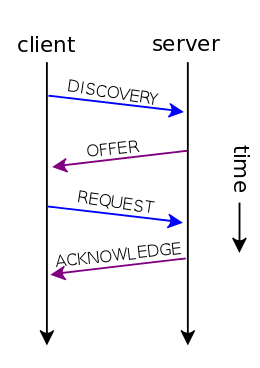
\includegraphics[scale=0.5]{images/dhcp.png}
\newline
\href{https://en.wikipedia.org/wiki/File:DHCP_session.svg}{\color{red}\textit{source: Wikipedia}}

Firstly, the client sends a Discover packet in order to notify the DHCP server it wants an ip address. Secondly, the server sends an Offer packet, which offers an ip address to the client. After recieving the Offer packet, the client sends a Request packet for the offered ip address. Lastly the server sends an Ack packet to confirm the ip address assignment of the client.
